\documentclass[UTF8]{article}
\usepackage{ctex}[14pt,a4paper]
\usepackage{graphicx}
\usepackage[left=4.2cm,right=4.2cm,top=3.5cm,bottom=3.5cm]{geometry}
\usepackage{epstopdf}
\usepackage{float}
\usepackage{threeparttable}
\usepackage{subfig}
\usepackage{amsmath}
\usepackage{cases}
\usepackage{url}
\usepackage{epstopdf}
\usepackage{float}
\usepackage{subfig}
\usepackage{amsmath}
\usepackage{cases}
\usepackage{geometry}
\geometry{left=1.3in,right=1.3in,bottom=1.25in}
\newcommand{\upcite}[1]{\textsuperscript{\textsuperscript{\cite{#1}}}}
\title{题目}
\date{}
\begin{document}

\section*{摘\quad 要}
\begin{flushleft}

		
		
\textbf{Key Words:} {}
\newpage
\end{flushleft}

\section{Restatement}
\subsection{Problem Background}

With the development of e-commerce and the improvement of the logistics service level, more and more people choose online shopping as a fast and convenient shopping method. With the development of big data and the massive increase of data, data plays an important role in business decision-making and company development. Customers can obtain information from other people's evaluations to decide whether to buy; companies can discover information from big data to better serve customers, increase efficiency, and enhance industry competitiveness.

\subsection{The Question Raised}

For Sunshine's three online sales products to succeed, we first need to identify key patterns, relationships, metrics, and parameters that are relevant through reviews and ratings in the only available data given. Then our two major goals are 1. To clarify the sales strategy; 2. To discover the important characteristics that potentially affect sales and help improve product satisfaction. Finally, a series of requirements should be fully considered;

\begin{itemize}

	\item Establish a data measurement mechanism: Once the hairdryer, microwave oven, and baby pacifier are sold online, the company can discover the product ’s customer preferences, sales, and areas worth improving based on market reactions (ratings, reviews).

	\item Taking the time factor into consideration and establishing a time-based model, we can discuss the future development trends of each commodity, market competitiveness, and market reputation.

	\item Combine text and rating metrics to predict whether a product will succeed in the market.


	\item Consider whether a particular star rating will trigger similar comments from others.

	\item Whether some special words are strongly related to ratings.

\end{itemize}

\subsection{Analysis}

First, we need to perform sentiment analysis and word frequency extraction on the comments through Python's natural language processing library. Then build a model for data mining of text and data, including product reputation, keywords, comment validity, and product characteristics. Finally, give Sunshine some online sales strategies.

\section{Assumption}

\begin{itemize}

	\item Suppose a user makes a review once they purchase a product, and the sales volume is considered to be equivalent to the number of reviews.

	\item Assume that the product data set provided by Sunshine is in line with the laws of the online market, that is, no abnormal conditions have occurred in the period of the data set, such as the increase or decrease in product sales caused by natural disasters.

	\item Suppose that the time interval between the user placing an order and receiving the goods in the data set is small, that is, the user comments shortly thereafter.

	\item Treat orders with significant differences in ratings and reviews as normal orders.

\end{itemize}

\section*{Symbol Description}
\begin{table}[h]
\centering

\begin{tabular}{lll}
	\toprule
	Symbol\ quad\quad\quad\quad\quad\quad\quad\quad\quad &Significance  \\
	\midrule
	$ \mathbf{k}  $   &  Review Score
	\\
	$ \mathbf{s}  $   & Star Rating
	\\
	$ \mathbf{P}  $   & Polarity Score
	\\
	$ \mathbf{S}  $   & Subjective Score
	\\
	$  \mathbf{\beta_i} $   & Helpfulness Rating
	\\
	$\mathbf{r}   $   & Importance of Reviews
	\\
	$ (\boldsymbol{f1},\boldsymbol{f2},\boldsymbol{f3})  $   & Review Score, Product Score, Consumer True Evaluation Score
	\\
	$  \mathbf{p} $   &Each Reviewer's Credit for the Product's Reputation
	\\
	$ \psi_j $   &  Product j Potential Score
	\\
	$  \rho $   & Person Correlation Coefficient
	\\	
	\bottomrule
\end{tabular}
\end{table}

\section{Model 1: Word Frequency Algorithm}
\subsection{Introduction and preliminary preparation of TF-IDF algorithm}

To determine the attribute information of each comment, we must first extract the valid information in the comment sentence. Then judge the words based on the extracted words. The TF-IDF algorithm is a statistical algorithm that can count the number of occurrences of a word in an article, and then find the frequency of the word. We use the frequency of words to characterize the importance of the word in the article.

Before performing word frequency statistics, we must also understand how computers extract words from articles. We know that extracting words is a very tedious task, and in the process, we have to consider multiple situations:

\begin{itemize}

	\item Some simple words such as $'a', 'an', 'is', 'the' \cdots$ exist in large numbers and have no analytical significance, so when natural language processing is performed, such words are not considered, so stop Words are not considered.

	\item For example, $'like'$, $'Like'$, and $likes$ have different capitalization and different word tenses. They should be regarded as one word, but they are treated as different words in this article for analysis.

	\item When segmenting sentences with spaces and punctuation to extract words, some abbreviations such as $we'll$, $we're$, $pinkish-blue$ were difficult to separate, but they can be accurately performed in the NKTL library Division.

\end{itemize}

Python has many very powerful natural language toolkits that can save us a lot of time with seemingly simple but very complex operations. On the processing of stop words, we downloaded a stop word dataset \url{https://blog.csdn.net/shijiebei2009/article/details/39696523/}, which contains 891 words. When processing text data, we deleted $891 * 2 + 1$ words from the divided words, which took into account the capitalization of stopword words and unexplained space characters.

In the word frequency algorithm, the reason why we use the NLTK library to implement the TF-IDF algorithm is that the NLTK library can process multiple text contents into a combined calculation instead of only a single text.

\subsection{TF is Term Frequency}

TF indicates how often the keyword appears in the text. To prevent it from biasing towards longer text, this number is usually normalized. It is worth mentioning that for other considerations later, we also use the word frequency. The formula is as follows:

\begin{equation}
t f_{i j}=\frac{n_{i, j}}{\sum_{k}^t n_{k, j}}
\end{equation}
where:

$n_ {i, j}$ represents the number of times the i-th word appears in the file $d_j$;

t represents the number of all entries in the file $d_j$

The denominator is the sum of the number of occurrences of all terms in the file $d_j$.

\subsection{IDF is Inverse Document Frequency}

 The main idea of TF-IDF is: if a word appears frequently in one article and rarely appears in other articles, it is considered that the word has good class discrimination ability and is suitable for classification. If fewer documents are containing the term t and the larger the IDF, it means that the term has good category discrimination ability \upcite{Baenagarc2012TF}. This is also in line with our goal of qualitative analysis of the evaluation content. The formula is as follows:

 \begin{equation}
 i d f_{i}=\log \frac{|D|}{\left|\left\{j: t_{i} \in d_{j}+1\right\}\right|}
 \end{equation}
 where:

 $|D|$ represents the number of texts studied;

 $j: t_{i} \in d_ {j}$ represents the number of files containing the term ti. Adding 1 here is to avoid the situation where the denominator is 0.

\subsection{TF-IDF is Actually: TF * IDF}

The high word frequency in a particular file and the low file frequency of the word in the entire file set can generate a high weighted TF-IDF. Therefore, TF-IDF tends to filter out common words and retain important words. The formula is:

\begin{equation}
TF-I D F=T F * I D F
\end{equation}

\subsection{How to Track Sales Situation form This Modle}

By understanding the frequency of occurrences and comments, we can understand that consumers really care about the characteristics of the product, and we can analyze and obtain the places where consumers are not satisfied with the products and sales services. Sunshine can improve and strengthen these places.

\section{Model 2: Evaluation Model Based on User Reviews}

\subsection{Qualitative Analysis of Reviews}

Today's online shoppers have different definitions of good or bad products, but unless shoppers are particularly dissatisfied with a product, most of the time they will praise it. Because online product providers do not have the cost of appearance fees, etc., the products on the Internet are very cheap, and people tend to be more "sympathetic" to a cheaply purchased product. Frequently "OK, OK, OK" reviews like \upcite{zz}. The content of the review is the data that determines the true thinking of the buyer. We need to mine the true score of the product from the text data.

\begin{figure}[h]
	\centering
	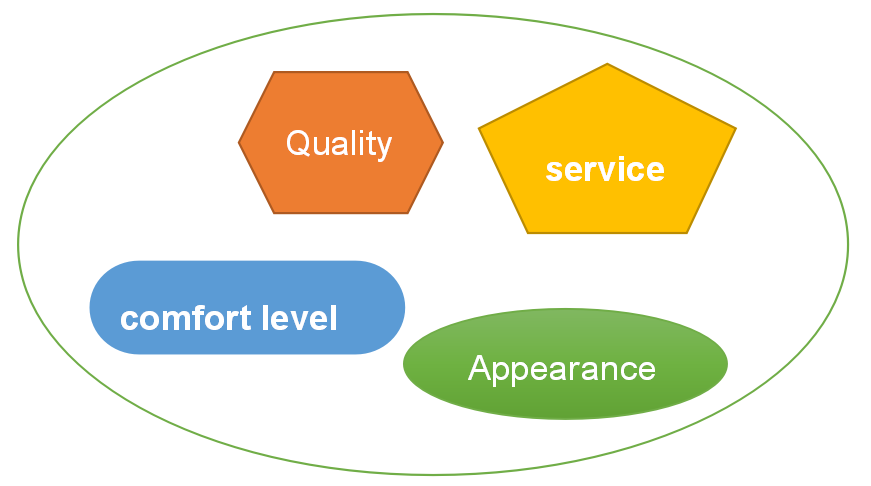
\includegraphics[width=6cm]{./figures/m1p.png}
	\caption{The main content of the product review} \label{m1p}
\end{figure}

As can be seen in figure \ref{m1p}, the main content of the review includes four aspects: quality, service, comfort, and appearance. A large number of reviews also include subjective feelings after using the product. Therefore, it is necessary to carry out a sentiment analysis of goods.

TextBlob stands on the huge shoulders of NLTK and pattern, and both work well together, and can be used for in-depth research on general natural language processing (NLP) tasks such as part-of-speech tagging, noun phrase extraction, sentiment analysis, etc. \upcite{Martinc2015Efficient }. Affective and subjective classification: This is the area most studied in academia. It treats sentiment analysis as a text classification problem. Two sub-themes that have been studied extensively are:(1) classify documents with opinions as expressing positive or negative opinions, (2) classify sentences or clauses as subjective or objective, and subjective sentences or clauses as positive, negative or Neutral perspective. Sentiment analysis aims to find the author's overall sentiment in the reviewed text. For example, given a product review, it determines whether the reviewer's sentiment about the product is positive or negative. In this article, we used sentiment analysis to get two values: polarity, subjectivity. polarity indicates that the polarity score floats in the range [-1.0, 1.0]. The subjective score is floating in the range of [0.0, 1.0], where 0.0 is very objective and 1.0 is very subjective.

This article divides all comments into 5 categories for analysis:

1. Praise (pure praise, without any bad words about the product);

2. Praise (overall praise, with some dissatisfaction);

3. Middle evaluation (more objective evaluation, centered view);

4. Negative evaluation (due to some unexpected or service attitude, such as express delivery reasons);

5. Negative evaluation (due to the product itself, such as quality reasons).

Perform a qualitative analysis of the review content by polarity and get a review score:

\begin{equation}\label{m1gs1}
k_i=\left\{\begin{array}{lll}
1 & \text { bed review } & \text {if -1 $\leq$ polarity < 0 }\\
2 & \text { medium review } & \text {if polarity = 0 }\\
3 & \text { good review } & \text {if 0 < polarity $\leq$ 0 }
\end{array}\right.
\end{equation}

\begin{figure}[!htbp]
	\centering
	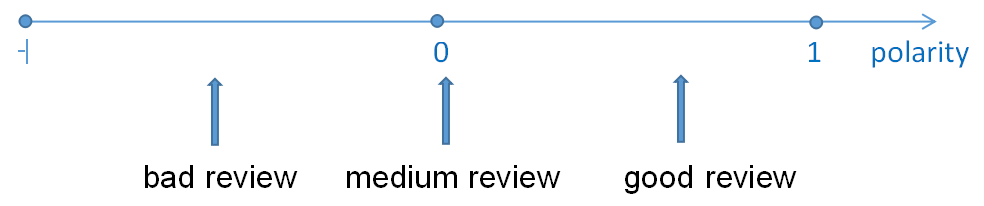
\includegraphics[width=8cm]{./figures/m11p.png}
	\caption{Attribute analysis of comment content} \label{m11p}
\end{figure}

$k_i$ is the review score, which is based on consumer reviews. polarity indicates that the polarity score floats in the range [-1.0, 1.0]. The closer the polarity is to the product of the 1st name, the better the product is, and the closer the polarity is to the -1 of the name, the worse the product is. 0 means that the consumer's review of the product is neither a negative review nor a positive review, that is, a middle review, with a rating of 2.

\subsection{Importance of Reviews}

The importance of comments is reflected in four aspects:

\begin{itemize}

	\item The larger the ratio of useful votes to the total votes, the greater the amount of information. Increase the importance by 1, but no more than 2;

	\item If the customer ’s rating is high and the label is “green label”, the influence is greater and the importance is increased by 2;

	\item If the customer's reviews are more objective, ie the subjectivity is smaller, the reviews are more important, and the importance is increased by 1;

	\item If the customer did buy the product, the review has higher credibility and an increase of 1.

\end{itemize}

Based on the above description, get the importance of the comment:

\begin{equation}
r_{i}=\frac{\sum_{1}^{4}r_{ij}}{\mathbf{max} r_i}
\end{equation}

\begin{equation}
\beta_i=\left\{\begin{array}{ll}
\frac{helpful\quad votes}{total\quad votes} & \text { if total votes $\neq$ 0 } \\
0 & \text { else }
\end{array}\right.
\end{equation}

Among them:

$\beta_i$ is the ratio of useful votes;

$
r_{i1}=\left\{\begin{array}{ll}
2 & \text { if $\beta_i$ > 50\% } \\
1 & \text { if $\beta_i \leq $50\% } \\
0 & \text { $\beta_i$ = 0 }
\end{array}\right.
$
represents the importance attribute of the useful ticket;

$
r_{i2}=\left\{\begin{array}{ll}
2 & \text { if vine = Y } \\
0 & \text { else }
\end{array}\right.
$
represents the important attribute of the reviewer;

$
r_{i3}=\left\{\begin{array}{ll}
1 & \text { if $S_i$ <0.5  } \\
0 & \text { else }
\end{array}\right.
$
represents the objective degree attribute of the review;

$
r_{i4}=\left\{\begin{array}{ll}
1 & \text { if verified purchase = Y } \\
0 & \text { else }
\end{array}\right.
$
represents the objective degree attribute of the review;

\subsection{Output Model for Different Information}

\begin{equation}\label{q1}
f(\boldsymbol{k},\boldsymbol{r},\boldsymbol{s})=(\frac{1}{3}\boldsymbol{k}^T\cdot \boldsymbol{r},\eta \boldsymbol{s} + 5(1-\eta)\boldsymbol{r},\phi\boldsymbol{s} + \frac{5}{3}(1-\phi)\boldsymbol{k})=(\boldsymbol{f1},\boldsymbol{f2},\boldsymbol{f3})
\end{equation}\label{zy1}
Where:

$f1_i$ represents the effective score of the review, ranging from $[0,1]$. This takes into account the review score obtained from the sentiment analysis of the text and the importance of the review. The effective score of reviews is to be able to filter out important reviews and is an important basis for providing customer opinions to Sunshine.

$f2_i$ represents the product score and ranges from $[0,5]$. Able to comprehensively reflect the value and quality of the product. This is essential for evaluating whether a product will succeed or fail. Because sometimes star ratings and reviews are contradictory, this is why we use a weighted method to coordinate the two. We know that reviews are entered manually, and it is impossible to violate the original evaluation of the consumer, and the star rating is clicked on the mouse, so it is likely to be wrong. A star rating of 1 or 2 appears, but reviews are good.

Why didn't we delete the data that star rating and review contradicted?

Because the data is given through the questions, we find that the data before 2008 are very small. If the original data is reduced, it is not good for data analysis.

$f3_i$ represents the true consumer evaluation score, ranging from $[0,5]$. This can reflect consumers' true feelings about buying products.

$\phi$ represents the weight of star ratings in consumers 'true evaluation scores, and $1- \phi$ represents the weight of review scores in consumers' true evaluation scores. In real consumer evaluation scores, we consider star ratings and evaluation scores to be equally important, so $\phi = 0.5$.

$\phi$ represents the weight of star rating in product score, and $1- \phi$ represents the weight of review score in product score. In product scores, evaluating effective scores is considered a more important factor than star ratings, so $\eta = 0.3$.

\subsection{How to Track Sales Situation form This Modle}

Once the three products are sold on the online market, Sunshine can measure and track product sales based on these three data. Sunshine Company can understand the pros and cons of the substantive factors such as product quality in the minds of consumers through product scores. It can also determine the true feelings of the product in the minds of consumers based on the true evaluation scores of consumers.

\section{Problem Results and Suggestions}

\subsection{Inform Online Sales Strategy}

First, we do some basic analysis of known raw data to understand the basics of online sales. Ask a series of questions that Sunshine may be interested in?

1. Is online shopping in the United States more and more common?

2. Will online sales replace traditional market sales?

3. Who has a better user experience compared to online sales?

4. What products are suitable for online sales?

5. What aspects of the product are consumers more concerned about?

\begin{figure}[h]
	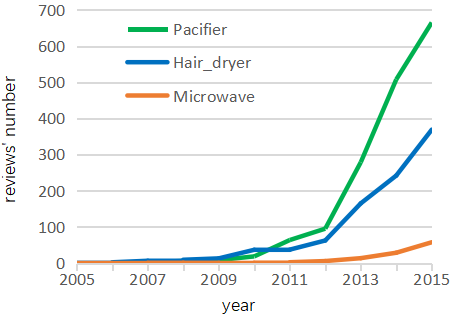
\includegraphics[width=7cm]{./figures/q1p1.png}
	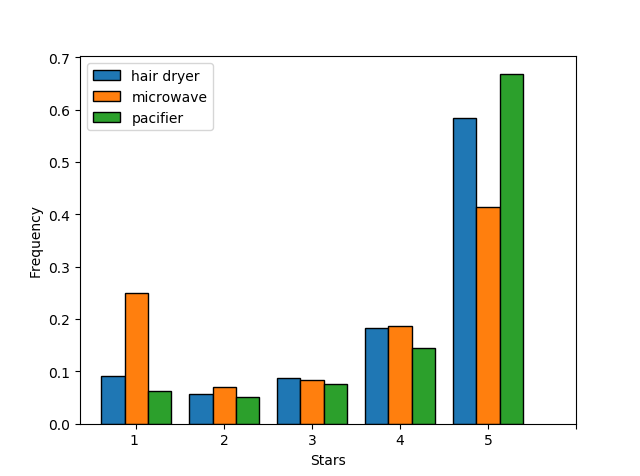
\includegraphics[width=7cm]{./figures/z1.png}
	\caption{Left: monthly average number of reviews for each of the three products; right: all data star frequency} \label{z1_q1p1}
\end{figure}

We know that the number of reviews is directly proportional to the number of online shoppers, so the picture on the right can be viewed as the relationship between online purchases and time. From the picture on the left, we can see that very few people chose to shop online before 2008, and online shopping has become more and more popular after 2008. Analyzing the reasons, the subprime mortgage crisis in the United States in 2008 triggered the global financial crisis, which led to the collapse of many banks and the impact of small and medium-sized enterprises. In order to survive, many small companies have turned to online sales because it is known that online sales costs are low No rent, GU sales staff.

We found that after 2008, the number of online shoppers has grown exponentially, which indicates that online shopping is becoming more popular with customers. We have reason to believe that online sales will defeat traditional market sales, and online shopping will become a new habit for people in the new era. It is strongly recommended that Sunshine Company develop an online sales business.

Pacifiers belong to the category of baby products, hairdryers belong to the category of beauty products, and microwave ovens belong to the category of large household appliances. In the picture on the left, we find that compared to hairdryers and pacifiers, the number of microwave oven reviews is very small, that is, fewer people buy microwave ovens online. Combined with the picture on the right, you can find that the one star of the microwave oven is very large, which shows that consumers do not like to buy large appliances on the Internet. In summary, beauty and baby products are more suitable for online sales.

The picture on the right is the distribution of star ratings for three categories of products. The five-star appearance of pacifiers and hair dryers is more than 50\%, indicating that most people have a good online shopping experience for these products. Everyone can buy things that are cheap and easy to use and can meet their needs.

TF-IDF algorithm is used to count the word frequency of the content of the review through Python's NLTK, and the following word cloud diagram is drawn by word cloud.
%%%%%%%%%%%%%%%%%%%%%%%%%%%%%%%%%%%%%%%%%%%%%%%%%%%%%%%%%%%%%%%%%%%%%%%%%%%%%%%%%%%%%%%%%%%%%%%%%%%%%%%%%%%%%%%%%%%%%%%%%%%%%%%%%%%%%%%x


\end{document}
